\chapter{Softwarearchitektur des Java Medical Imaging Toolkit} \label{architecture}

\section{Die Eclipse Rich Client Platform}

Die Grundlage für eine modulare Entwicklung der Software liefert die Eclipse Rich Client\footnote{Es lässt sich zwischen Rich Clients und Thin Clients unterscheiden. Rich Clients stellen sowohl die Präsentationsschicht als auch die logische Schicht auf dem Client zur Verfügung. Die Applikationsfunktionalität der Thin Clients wird komplett von einem Server bereitgestellt. Die Bedienung erfolgt meist über den Browser.} Platform (RCP). Eclipse, basierend auf der Programmiersprache Java, wird seit 2001 von einer OpenSource-Gemeinde entwickelt\cite{vogel:eclipseoverview}. Während es Anfangs rein für die Java-Applikationsentwicklung entworfen wurde, ist es heute eine allgemeine erweiterbare Entwicklungsumgebung. So lässt sich zum einen das Grundprogramm mit Hilfe sogenannter Plug-ins erweitern und zum anderen eigenständige Applikationen erstellen (RCP), die auf dem Eclipse-Framework aufbauen. Das \glqq Aptana Studio\footnote{http://www.aptana.com/}\grqq\ ist beispielsweise ein Plug-in, das der Grundentwicklungsumgebung mehrere Funktionalitäten im Bereich der Webentwicklung (Kommunikation zum Server, Syntaxhighlighting von HTML und CSS) hinzufügt. RSS Owl\footnote{http://www.rssowl.org/}, ein Programm zur Verwaltung von Newsfeeds, ist ein Beispiel für eine eigenständige Rich Client Applikation auf Basis von Eclipse.\\
Eine Kernkomponente des Eclipse-Frameworks ist \textit{Equinox}, eine Implementierung der OSGi-Spezifikation. OSGi bietet die Möglichkeit, modulare Java-Applikationen zu entwickeln und Softwarepakete (nach der Spezifikation \glqq Bundles\grqq\, unter Eclipse \glqq Plug-ins\grqq\ genannt) während der Laufzeit hinzuzufügen, zu entfernen, zu starten oder zu stoppen \cite{vogel:e4overview}. Das Java Medical Imaging Toolkit ist eine Implementierung eines Bundles beziehungsweise Plug-ins.\\
Abbildung \ref{eclipsee4arch} zeigt die Architektur der Eclipse Rich Client Platform.

\begin{figure}[htbp]
  \vspace{0.5cm}
  \centering
  \fbox{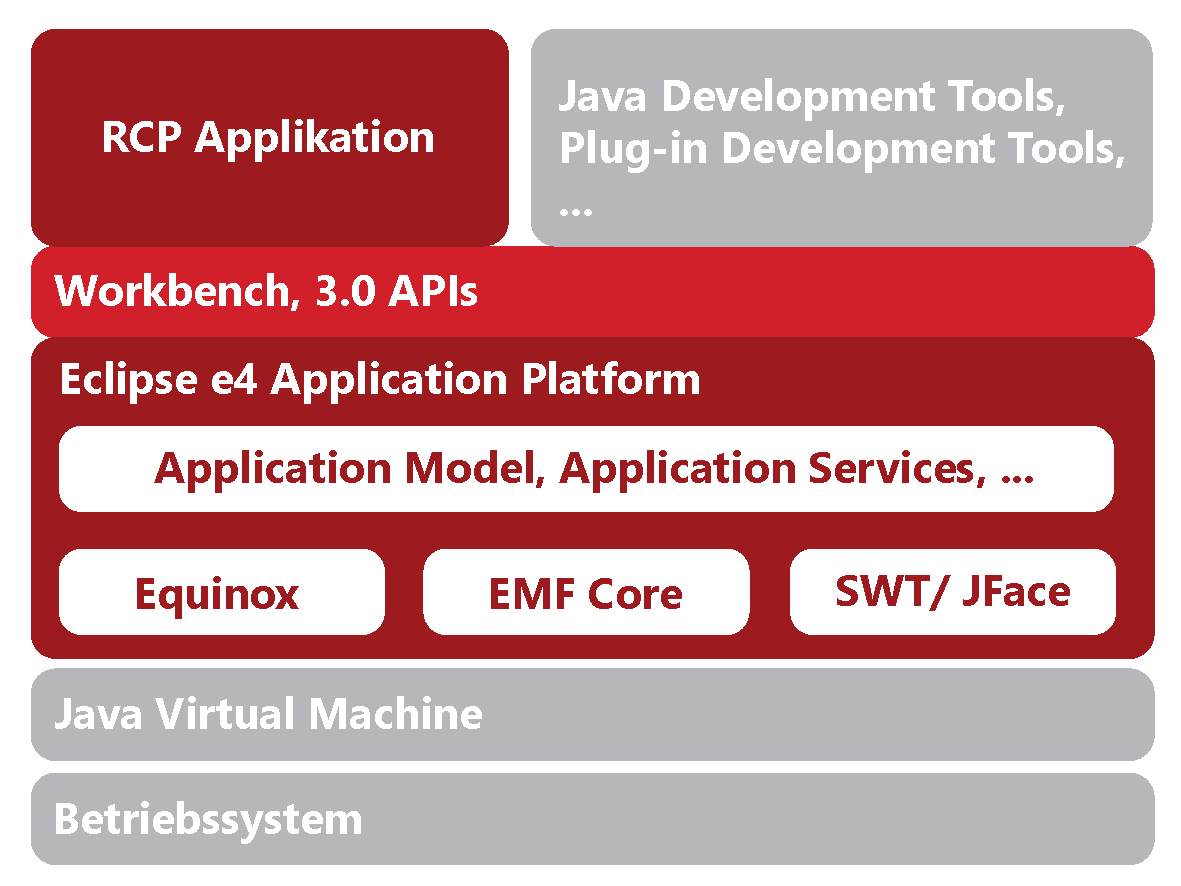
\includegraphics[angle=0,width=10cm]{./img/e4arch.pdf}}
  \caption{Architektur der Eclipse e4 Plattform zur Entwicklung von Rich Client Applikationen}
  \floatfoot{https://wiki.eclipse.org/Eclipse4}
  \label{eclipsee4arch}
  \vspace{0.5cm}
\end{figure}

Die untere Ebene bildet das Betriebssystem. Eclipse kann grundsätzlich plattformunabängig unter Windows, verschiedener Linux Distributionen oder Mac OS eingesetzt werden. Einzige Voraussetzung ist eine installierte Java Virtual Machine. Aufbauend auf Java steht der Eclipse-Kern, bestehend aus dem OSGi-Framework Equinox, dem Eclipse Modeling Framework EMF\footnote{Das EMF dient beispielsweise zur Entwicklung eines Datenmodells, wird allerdings für weitere Ausführungen nicht explizit benötigt.} und dem Standard Widget Toolkit SWT. Das SWT ist eine OpenSource Implementierung verschiedenster grafischer Bedienelemente wie Schaltflächen, Textfelder, Tabellen und vieles mehr.Der Unterschied zu den in Java integrierten grafischen Oberflächen besteht darin, dass das Standard Widget Toolkit auf die Ressourcen des Betriebssystems zugreift und sich in der Darstellung den Betriebssystemstandards anpasst\cite{eclipse:swt}. Aufbauend auf den Grundkomponenten liegt das \textit{Application Model}, das die Struktur der Applikation(Menüs, Fenster, etc.) beschreibt \cite[Kapitel 7]{vogel:e4overview}. Workbench und Eclipse 3.0 APIs bieten noch die Möglichkeit Anwendungen abwärtskompatibel zu entwickeln. Die gesamte Plattform bildet die Basis für das Java Medical Imaging Toolkit. Durch das Application Model kann modular entwickelt und die Programmstruktur in zukünftigen Versionen erweitert werden.

\section{Das Eclipse Application Model}

Damit eine Anwendung strukturiert werden kann stellt das Application Model steuernde und visuelle Elemente zur Verfügung.
\begin{itemize}

\item \textbf{Strukturen zur visuellen Beschreibung der Applikation}\\
	Das Aussehen wird mit Hilfe von Windows, Parts, PartStacks und Anderen beschrieben. Die Elemente enthalten noch keine Logik sondern definieren nur die Struktur der Anwendung.


\item \textbf{Strukturen zur Steuerung des Verhaltens}\\
	 Zu den Komponenten, die das Verhalten der Applikation beeinflussen zählen zum Beispiel Tastatur-Shortcuts, Commands und Handler. Letztere dienen zur Verarbeitung von Benutzereingaben.

\end{itemize}

\subsection{Visuelle Komponenten}

\subsubsection{Window}
Windows sind einfache Repräsentationen eines Fensters der Benutzeroberfläche\cite[org.eclipse.e4.ui.model.application.ui.basic]{eclipse:help}. Sie bilden das Grundgerüst der Applikation und beinhalten Perspectives, PartStacks und andere Elemente. Ein einfaches Fenster ist in Abbildung \ref{rcp_window} zu sehen.

\subsubsection{Menüs}
Ein Menü ist der Container für verschiedene Menü-Elemente und dient dazu Benutzereingagen entgegenzunehmen. Einem Element können Commands hinterlegt werden, damit die Eingaben weiter verarbeitet werden können. Ein Menüpunkt kann selbst ein Menü beinhalten.

\subsubsection{Perspective}
Perspectives beinhalten eine Menge von Elementen der Benutzeroberfläche wie PartStacks und Parts. Perspectives können unabhängig vom Rest der Oberfläche gewechselt werden\cite[org.eclipse.e4.ui.model.application.ui.advanced]{eclipse:help}. So können Perspectives beispielsweise die Anordnung der Parts definieren, oder neue Parts anzuzeigen, die in einer anderen Perspective nicht zu sehen sein sollen. Unter Eclipse hat zum Beispiel der Debug-Modul eine eigene Perspective und es kann dynamisch zwischen Debug- und Entwicklungsperspektive gewechselt werden.

\subsubsection{PartSashContainer}
Wie der Name bereits andeutet, ist ein PartSashContainer ein Container für PartStacks und Parts. Die enthaltenen Elemente werden komplett angezeigt. In Abbildung \ref{rcp_partsash} ist eine solche Kombination zu sehen. Die obere Hälfte stellt einen PartStack mit den beiden Parts \textit{TestPart A} und \textit{TestPart B} dar. Der Untere Teil ist ein Stack-unabhängiger Part.

\subsubsection{PartStack}
Auch der PartStack dient als Behälter für einzelne Parts. Der Unterschied zum PartSashContainer liegt darin, dass bei PartStacks nur der aktuell ausgewählte Part angezeigt wird. Die Darstellung des Stacks ist mit üblichen Tabs zu vergleichen, wie Abbildung \ref{rcp_partStack} zeigt. Der Stack enthält die beiden Parts \textit{TestPart A} und \textit{TestPart B}.

\subsubsection{Part}
Ein Part ist die kleinste Einheit des Application Models und ist Kern der Benutzeroberfläche\cite[org.eclipse.e4.ui.model.application.ui.basic]{eclipse:help}. Innerhalb der Parts werden alle weiteren Bedienelemente angezeigt. Jede Abbildung von \ref{rcp_part} - \ref{rcp_partsash} enthält eine oder mehrere Parts. Betrachtet man das Application Model als Baumstruktur, symbolisieren Parts die Blattknoten. Parts können direkt einem Window unterstellt oder tief verschachtelt zwischen Perspectives und Stacks benutzt werden.


\subsection{Steuernde Komponenten}
\subsubsection{Commands}
Commands bilden die abstrakte Schicht zwischen Benutzereingabe und Verarbeitung. Commands besitzen keine eigenen Implementierung. Das ermöglicht dem Entwickler das Verhalten indiviuell zu gestalten. So könnte ein Einfügen-Befehl im Editor ein anderes Verhalten auslösen als im Explorer-Part\cite[org.eclipse.ui.commands]{eclipse:help}.

\subsubsection{Handler}
Handler sind die konkreten Implementierungen der Commands und sind für die Verarbeitung der Benutzereingaben verantwortlich.

\begin{figure*}
%\subfigure[Keypoints]{\includegraphics[width=0.49\textwidth]{./img/basmati_keypoints.png}}\hfill
%\centering

\subfigure[Window]{\includegraphics[width=0.40\textwidth]{./img/rcp_window.png} \label{rcp_window}}\hfill
\subfigure[Part]{\includegraphics[width=0.40\textwidth]{./img/rcp_part.png} \label{rcp_part}}\\
\subfigure[PartStack]{\includegraphics[width=0.40\textwidth]{./img/rcp_partStack.png} \label{rcp_partStack}}\hfill
\subfigure[PartSashContainer]{\includegraphics[width=0.40\textwidth]{./img/rcp_partsash.png} \label{rcp_partsash}}

\caption{Verschiedene Elemente des Application Models}
\label{rcp_example}
\end{figure*}

\section{Die Benutzeroberfläche von jMediKit}

Die Oberfläche des Java Medical Imaging Toolkit besteht aus sechs zentralen Elementen.
\begin{enumerate}
\item \textbf{Hauptmenü} \\
	  Das Hauptmenü stellt globale und bildspezifische Operationen zur Verfügung. So werden unter dem Menüpunkt \textit{Erweiterungen} die importierten Plug-ins aufgelistet.
\item \textbf{Werkzeugleiste} \\
	  Dieser Teil der Benutzeroberfläche stellt hauptsächlich Möglichkeiten zur Manipulation der Bilddaten zur Verfügung. Das Kapitel \glqq \ref{implementation}. \nameref{implementation}\grqq\ geht genau auf die verfügbaren Werkzeuge ein.
\item \textbf{DicomBrowser} \\
	  Dieser Part erlaubt die Navigation durch die vom Programm geladenen DICOM-Objekte. Die Anordnung entspricht der Darstellung des ER-Modells aus Kapitel \glqq \ref{grundlagen}. \nameref{grundlagen}\grqq\
\item \textbf{ImageView} \\
	 ImageView übernimmt die Anzeige der Pixeldaten der DICOM-Objekte.
\item \textbf{Console} \\
	Die Konsole dient für die Fehlerausgabe bei der Plug-in-Entwicklung.
\item \textbf{DicomTagView} \\
	Im DicomTagView werden die Tags eines ausgewählten DICOM-Objekts dargestellt.
\end{enumerate}

\begin{figure}[htbp]
  \vspace{0.5cm}
  \centering
  \fbox{\includegraphics[angle=0,width=12cm]{./img/jmedikit_ui.png}}
  \caption{Die Benutzeroberfläche von jMediKit}
  %\floatfoot{https://wiki.eclipse.org/Eclipse4}
  \label{jmedikitui}
  \vspace{0.5cm}
\end{figure}

Die hierarchische Struktur der Anwendung wird in Abbildung \ref{hierarchy} dargestellt. Die sechs Blattknoten repräsentieren die nach außen für den Benutzer sichtbaren Teil der Anwendung. 


\section{Erweiterbarkeit der Grundstruktur}
Die flexible Struktur des Eclipse Application Models und der Rich Client Platform erlauben komfortable Erweiterungen. So können einzelne Parts den schon bestehenden Elementen zugeordnet, oder neue Perspectives eingefügt werden. Beispielsweise könnte ein neuer Part den FileStack(Abbildung \ref{hierarchy}) damit erweitern, dass DICOM-Objekte von einem PACS geladen werden. Das Kapitel \glqq \ref{extending}. \nameref{extending}\grqq\ zeigt eine Möglichkeit, jMediKit einen neuen Part hinzuzufügen.\\
Damit ist der Teil erfüllt, dass die zu entwickelnde Anwendung für Erweiterungen offen steht. Modulare Werkzeuge komplettieren die Anforderung der Erweiterbarkeit für Entwickler.

\tikzstyle{every node}=[draw=black,thick,anchor=south, align=center]
%\tikzstyle{selected}=[draw=red,fill=red!30]
\tikzstyle{optional}=[dashed,fill=gray!50]
\begin{figure}[htbp]
\centering
\caption{jMediKit und die hierarchische Anordnung der Elemente des Application Models}
\label{hierarchy}
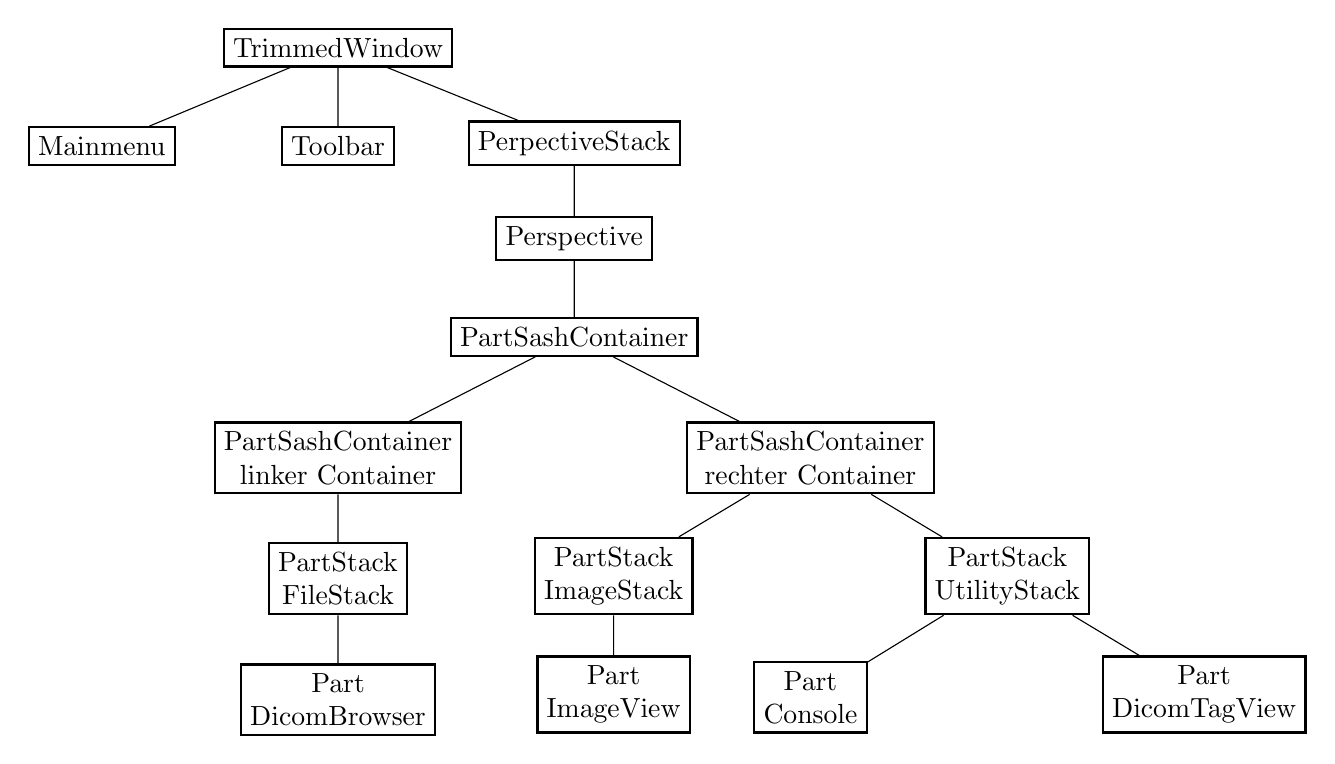
\begin{tikzpicture}[level distance=1.5cm,
  level 1/.style={sibling distance=3cm},
  level 2/.style={sibling distance=5cm},
  level 4/.style={sibling distance = 6cm, level distance = 2cm},
   level 5/.style={sibling distance=5cm},]
  \node {TrimmedWindow}
  child { node{Mainmenu}}
    child { node{Toolbar}}
    child {node {PerpectiveStack}
      child {node{Perspective}
      	child{node{PartSashContainer}
      	  child{node{PartSashContainer \\ linker Container}
      	    child{node{PartStack \\ FileStack}
      	      child{node{Part \\ DicomBrowser}}
      	    }
      	  }
      	  child{node{PartSashContainer \\ rechter Container}
      	    child{node{PartStack \\ ImageStack}
      	      child{node{Part \\ ImageView}}
      	    }
      	    child{node{PartStack \\ UtilityStack}
      	      child{node{Part \\ Console}}
      	      child{node{Part \\ DicomTagView}}
      	    }
      	  }
      	}
      }
    };
\end{tikzpicture}
\end{figure}

\section{Modulare Werkzeuge}

\section{Externe Bibliotheken}

\subsection{dcm4che}

\subsection{Java Advanced Imaging}

\section{Bibliotheken zur Plug-in Entwicklung}